\chapter{Clustering Techniques}
\label{chapter:clustering}

%Describe our basic assumption of function decomposition.
%Each subproblem should be composed of an observalbe uni-model.
We are interested in solving real-valued multimodal problems composed of observable unimodals.
Given the case, it is easier to solve an isolated unimodal within a subspace,
than tackling the complete search space with the multimodal problem.
Therefore, the first thing for solving a multimodal problem is to identify and isolate 
the potential uni-modals within the given search space.

%We wish to identify these uni-models through clustering techniques. 
We tried to isolate potential \textit{fitness hills}, i.e. uni-modals,
by clustering the initial samples points,
and consider each cluster as a multi-dimension normal distribution.
Different clustering techniques are often applied to identify different characteristics of clusters.
Here we proposed a \textit{hierarchical clustering} techniques to identify \textit{fitness hills},
since we consider not only the density of the particles,
but also the fitness values of different search points.
Our basic assumption for the under lying uni-modal is a weighted normal distribution, 
since we need to take fitness into account instead of viewing each point with the same weight.
We tend to focus on the particles with better fitness,
than a dense cluster with less fitness. 
It is also easier to calculate the weighted mean vector and weighted covariance matrix in higher dimension. 

Later, we applied the Minimum Description Length (MDL) to reduce the number of clusters.
Although a complex Gaussian Mixture Modal is able to describe the sample distribution better,
we believe that a more compact model, in terms of information entropy, is the better choice 
when multiple models can describe the same distribution. 
This also allows us to define a more stable subspace for further searching.


\section{K-Means Clustering}
In this section, we first describe the K-Means clustering techniques and its limitation for identifying the fitness hills.
K-Means clustering aims to partition $n$ observation data points into $k$ clusters.
There are two main procedures for K-Means clustering: the \textit{assignment} step and the \textit{update} step.

During the \textit{assignment} step, an initial set of $k$ means positions are given.
Then, each data point is assigned to the cluster with the \textit{nearest mean}.
The assignment to the \textit{nearest mean} can be formally described 
as creating clusters whose mean yields the least within-cluster sum of squares (WCSS), i.e. the sum of squared Euclidean distance.
During the \textit{update} step, the new centroids of each new clusters are calculated and assigned as the new means.
This can be also be described as minimizing the within-cluster sum of squares (WCSS).
The algorithm proceeds by alternating between these two steps until the means no longer change.
Since there only exists a finite states of partitions, the algorithm must converge to a local optimum.
However, different initial mean positions results in different clusters.

One of the main problem for using the K-Means clustering to identify \textit{fitness hills} is that
it considers only the spatial density and does not utilize the fitness value of each particle.
This results in different clusters each centering at a point that does not necessarily possess the best fitness in the neighborhood.
Therefore, the K-Means clustering often results in unstable clusters depending on initial conditions, and is highly sensitive to particle density.
Another common phenomenon for being sensitive to spatial density is that 
the points on the border of clusters might belong to different clusters after each update.
This makes the clusters unstable and costs unnecessary evaluations and computation for redefining the borders of ROI after each update. 

The other problem for using the K-Means clustering is that one needs to decide the number of clusters.
Determining the number of clusters is also a highly studied subjects, 
such as the silhouette coefficient~\cite{}, the Gap statistics~\cite{}, and the Dip-test~\cite{}.
Describe how silhouette score decides number of clusters 
Describe how gap statistics estimates number of clusters.
Describe how Dip-test checks unimodality

In the beginning particles should gather around the good solutions and gives a clear density signal
However, most of these techniques consider only the spatial density of points.




Figure~\ref{fig:Clustering_comparison} shows how K-Means fails to identify a uni-modal and results in four clusters due to density.
We would like our clustering method to be capable of identifying the uni-modal and be able to center around the particle with the best fitness.
Therefore, we adopted the weighted normal distribution as the underlying model. 


Describe how K-means clustering works and why it is popular Describe the limits for K-Means clustering, 
e.g. it cannot identify density nor unimodality.  

\begin{figure} 
\centering
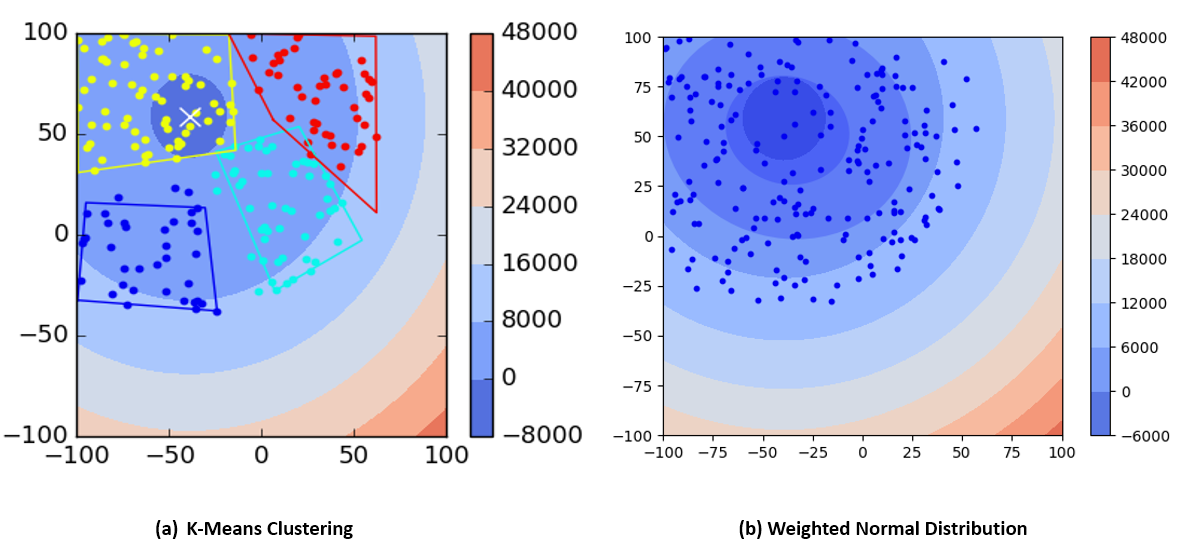
\includegraphics[width=\textwidth]{Clustering_comparison} 
\caption{Comparing K-Means clustering with weighted Gaussian Distribution on CEC2005 F1 Problem}\label{fig:Clustering_comparison}
\end{figure}

\begin{figure}
\centering
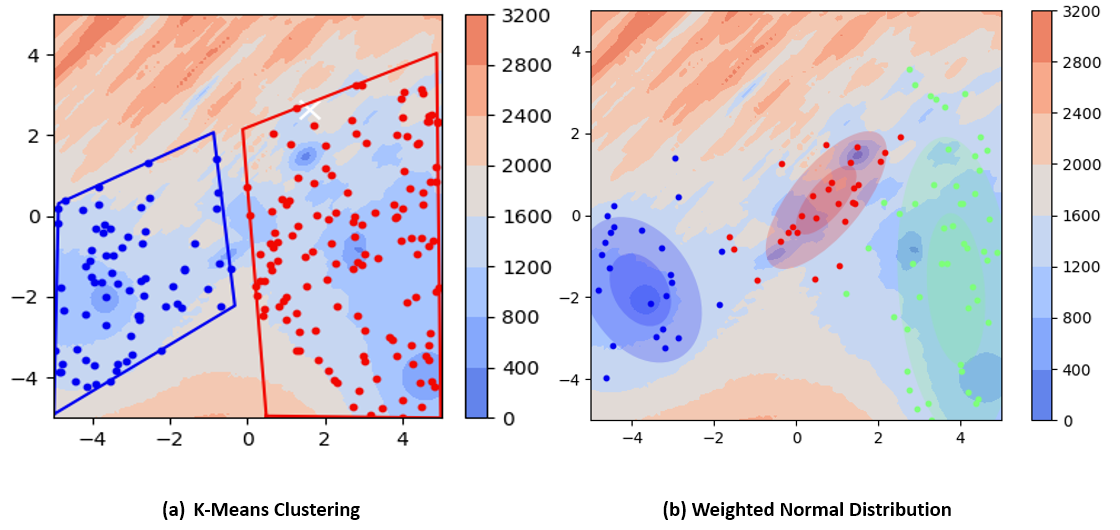
\includegraphics[width=\textwidth]{Clustering_comparison_F19}
\caption{Comparing K-Means clustering with weighted Gaussian Distribution on CEC2005 F19 Problem}\label{fig:Clustering_comparison_F19}
\end{figure}


\section{Heirarchical Clustering}
Describe the advantage of considering fitness instead of just density.



\section{Minimum description length and weighted multivariate normal distribution}

MDL~\cite{Rissanen:1984:Universal}.

KMDL~\cite{Kyrgyzov:2007:KMDL}

\begin{figure}
\centering
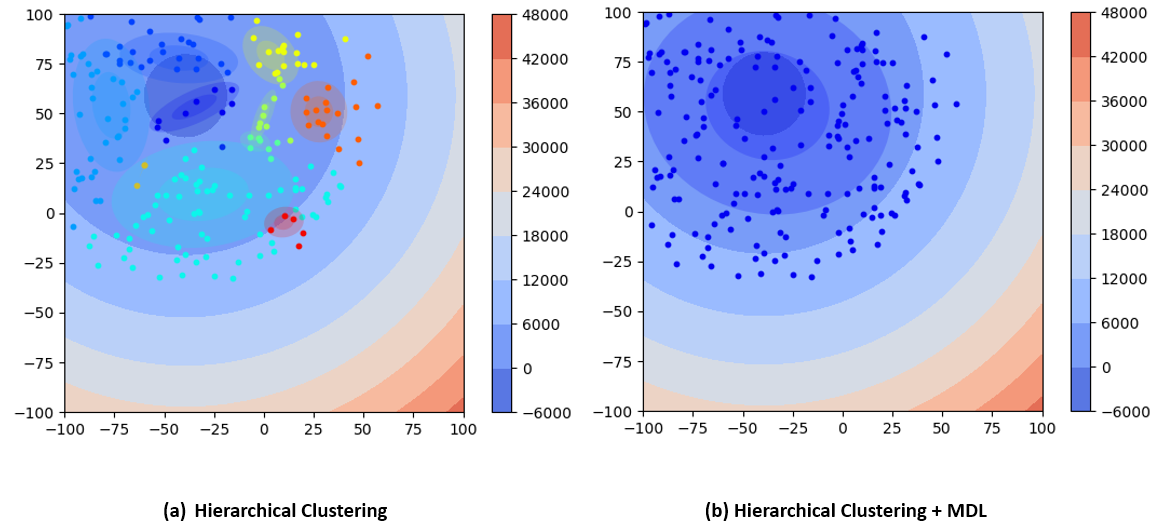
\includegraphics[width=\textwidth]{MDL_comparison}
\caption{Before and after Minimal Description Length trimming on CEC2005 F1 Problem}\label{fig:MDL_comparison}
\end{figure}

\begin{figure}
\centering
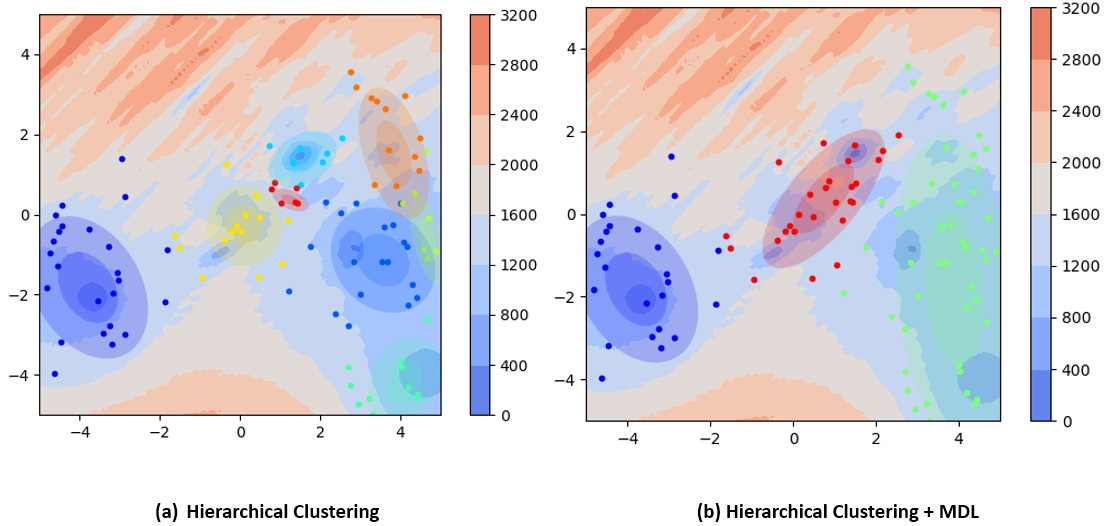
\includegraphics[width=\textwidth]{MDL_comparison_F19}
\caption{Before and after Minimal Description Length trimming on CEC2005 F19 Problem}\label{fig:MDL_comparison_F19}
\end{figure}






